\documentclass[10pt,a4paper]{article}
\usepackage{tikz, hyperref, graphicx, float}
\usepackage{etoolbox, needspace}

\de{\usepackage[german]{babel}}
\en{\usepackage[english]{babel}}

\de{\title{Entwicklerdokumentation für Ortungssimulator}}
\en{\title{Developer Documentation for Location Simulator}}

\en{\graphicspath{{../../fastlane-screenshots/en-US/images/phoneScreenshots}}}
\de{\graphicspath{{../../fastlane-screenshots/de-DE/images/phoneScreenshots}}}

\newcommand{\subsubsubsection}[1]{\paragraph{#1}\mbox{{}\\}}
\setcounter{secnumdepth}{4}
\setcounter{tocdepth}{4}

%Try to have subsubsections not start right at the end of a page, only used in ProjectStructure
\newlength{\sectionbuffer}
\setlength{\sectionbuffer}{0.0\textheight}
\pretocmd{\subsubsection}{\needspace{\sectionbuffer}}{}{}

\begin{document}
	
	\maketitle
	
	\tableofcontents
	
	\en{
\section{Installation}
To work with this project, clone the repository. It is recommended to do this manually and not with a tool like Android Studio, as the root of the gradle project is not the very first folder, but instead the android-app folder contained in it.

To now work with the project, open the android-app folder as a new project in Android Studio. Android Studio should now automatically guide you through the rest of the setup and install all dependencies.
}

\de{
\section{Installation}
Um an diesem Projekt zu arbeiten, klone das Git Repository. Dies sollte manuell geschehen, und nicht via Android Studio, da der root Ordner des gradle Projekts nicht der oberste Ordner ist, sondern der enthaltene android-app Ordner.

Um an dem Projekt zu arbeiten, öffne den android-app Ordner al ein neues Projekt in Android Studio. Android Studio sollte dich jetzt durch die weitere Einrichtung führen und alle Abhängigkeiten automatisch installieren.
}
	%TODO how did we call them?
\en{
\section{General Information}
\subsection{Architektur}
This app uses the Model View ViewModel (MVVM) architecture, which is a common architecture, splitting the software into three layers:
\begin{itemize}
	\item \textbf{The Model} contains the data, which can be modified by the ViewModel. The data is independent of the other layers, meaning multiple views implementations can use the same model. It might also contain some business logic, like accessing the devices main memory. For this project, the Models will be called XYZState.
	\item \textbf{The ViewModel} takes user inputs from the View and modifies the models data accordingly. It also iffer the view access to the state of the model, so any changes can be reflected in the UI. For this project, the View Models will be called XYZViewModel, with event that can happen being called XYZEvent.
	\item \textbf{The View} reacts to changes in the ViewModel and reflects those changes in the UI. It should contain no business logic. For this project, the Views will be called XYZScreen.
\end{itemize}
This architecture was used as the apps UI used Jetpack Compose, which is made to work with a ViewModel. The separation of the layers also allows for independent changes between UI and business logic, as well as bester testability, as no complex UI tests are needed to test the business logic.

\subsubsection{Data Bindings}
For databindings, Jetpack Compose already provides states that take care of updating and recomposing the UI.

\subsubsection{Further Resources}
\href{https://www.youtube.com/watch?v=8YPXv7xKh2w}{This YouTube video} further explains the MVVM architecture and was used by the developers of this app to learn it.

}


\de{
\section{Allgemeine Informationen}
\subsection{Architektur}
Diese App nutzt die Model View ViewModel Architektur, eine weiterverbreite Architektur, welche die Software in drei Schichten unterteilt:
\begin{itemize}
	\item \textbf{Das Model} enthält die Daten, die vom ViewModel modifiziert werden können.  Die Daten des Models sind unabhängig von den anderen Schichten und können daher von unterschiedlichen View Implementierungen verwendet werden. Es kann auch Geschäftslogik in dem Model liegen, wie das Einlesen von Daten aus dem Speicher.
	\item \textbf{Das ViewModel} nehmen Eingaben der UI über den View entgegen und modifizieren ggf. die Daten des Models. Sie bieten dem View einen State des Models, sodass die UI bei einer Änderung dieses States angepasst werden kann.
	\item \textbf{Der View} reagiert auf Änderungen des ViewModels und stellt diese in der UI da. Der View enthält keine Geschäftslogik.
\end{itemize}
Diese Architektur wird verwendet, da die UI der App mit Jetpack Compose entwickelt wurde, welches auf die Verwendung mit einem ViewModel ausgelegt ist. Des weiteren erlaubt die klare Trennung der Schichten eine unabhängige Entwicklung von UI und Geschäftslogik und erlaubt ein testen der Geschäftslogik ohne komplexe UI Tests.

\subsubsection{Datenverbindungen}
Jetpack Compose kommt bereits mit fertigen Datenverbindungen, welche dafür sorgen das UI und Model entsprechend der Änderungen angepasst werden.

\subsubsection{Weitere Ressourcen}
\href{https://www.youtube.com/watch?v=8YPXv7xKh2w}{Dieses Youtube Video} erklärt die MVVM Architektur im Detail und wurde von den Entwicklern dieser App verwendet, um die Architektur zu lernen.
}

\begin{figure}
	\centering
	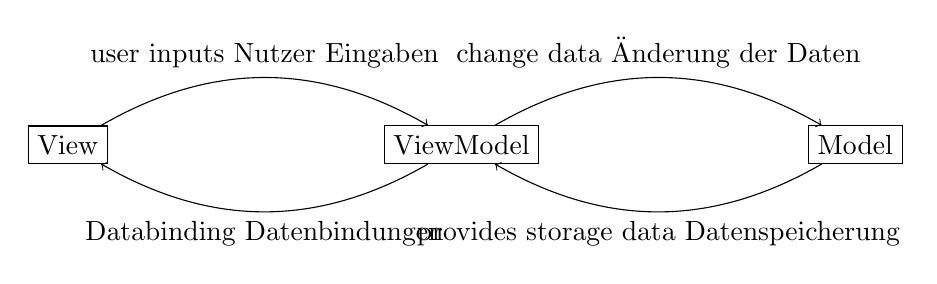
\begin{tikzpicture}[node distance=5cm]
		% Nodes
		\node (View) [draw, rectangle] {View};
		\node (ViewModel) [draw, rectangle, right of = View] {ViewModel};
		\node (Model) [draw, rectangle, right of = ViewModel] {Model};
		
		% Arrows
		\draw[->] (View) to[bend left] node[midway, above] {\en{user inputs} \de{Nutzer Eingaben}} (ViewModel) ;
		\draw[<-] (View) to[bend right] node[midway, below] {\en{Databinding} \de{Datenbindungen}} (ViewModel) ;
		\draw[->] (ViewModel) to[bend left] node[midway, above] {\en{change data} \de{Änderung der Daten}} (Model) ;
		\draw[<-] (ViewModel) to[bend right] node[midway, below] {\en{provides storage data} \de{Datenspeicherung}} (Model) ;
	\end{tikzpicture}
	\caption{\en{Overview of the MVVM architecture} \de{Überblick über die MVVM Architektur}}
	\label{fig:MVVM}
\end{figure}
	\setlength{\subsectionbuffer}{0.3\textheight}

\newcommand{\includefastlane}[1]{\includegraphics[width=0.3\textwidth]{
		\en{../../fastlane-screenshots/en-US/images/phoneScreenshots/#1}
		\de{../../fastlane-screenshots/de-DE/images/phoneScreenshots/#1}
		}}

\section{\en{Project Structure} \de{Projektaufbau}}
\en{The following section refer to all the packages found in\\ android-app/app/src/main/java/com/ispgr5/locationsimulator.}
\de{Die folgenden Abschnitte beziehen sich auf die Packages, die in\\ android-app/app/src/main/java/com/ispgr5/locationsimulator gefunden werden können.}

\subsection{core.util}
\begin{figure}[H]
	\centering
	\includegraphics[width=\textwidth, height=0.4\textheight, keepaspectratio]{img/core.util}
\end{figure}
\begin{itemize}
	\item \textbf{TestTags} \en{Contains all the test tags which can be used to test the app with it's UI. The most common use cases would be to check if a UI element exists, to get it's value or to click on it.} \de{Enthält alle Test Tags die verwendet werden können, um die App über ihre UI zu testen. Typische Verwendungsfalle wären um zu überprüfen, ob ein UI Element existiert, um seinen Wert zu erhalten, oder um auf es zu klicken.}
\end{itemize}

\subsection{data}
\en{This package contains a variety of classes for working with the database.} \de{Enthält eine Vielzahl an Klassen, um mit der Datenbank zu arbeiten.}

\begin{figure}[H]
	\centering
	\includegraphics[width=\textwidth, height=0.4\textheight, keepaspectratio]{img/data}
\end{figure}
\subsubsection{repository}
\begin{itemize}
	\item \textbf{ConfigurationRepositoryImpl} \en{Implements all the function that can be called to read configurations from the database, or write them to it.}
	\de{Implementiert alle Funktionen, mit denen Konfigurationen von der Datenbank gelesen oder auf die Datenbank geschrieben werden können.}
\end{itemize}

\subsubsection{source}
\begin{itemize}
	\item \textbf{ConfigurationDao} \en{Data Access Object for the Database where SQL queries are defined.} \de{Data Access Object fü die Datenbank, welches die SQL Queries definiert, um auf die Datenbank zuzugreifen.}
	\item \textbf{ConfigurationDatabase} \en{Defines the database which stores the configurations.} \de{Definiert die Datenbank, welche die Konfigurationen speichert.}
\end{itemize}

\subsubsection{storageManager}
\begin{itemize}
	\item \textbf{ConfigurationStorageManager} \en{This class is responsible for importing and exporting configurations. It turns sound files into a base64 string, creates a json for the configuration, and compresses them using gzip.} \de{Diese Klassen stellt die Funktionalitäten fü das Importieren und Exportieren von Konfigurationen zur Verfügung. Dabei werden Audio Dateien in Base64 Strings umgewandelt und die Konfiguration in eine JSON Datei verwandelt, welche mit GZIP komprimiert wird.}
	\item \textbf{SoundStorageManager} \en{This class allows us to use the sound files, which are stored on the devices main storage.} \de{Diese Funktion ermöglicht es uns die Audio Dateien zu verwenden, welche auf dem Hauptspeicher des Geräts gespeichert sind.}
\end{itemize}

\subsection{di} \label{sec:di}
\begin{figure}[H]
	\centering
	\includegraphics[width=\textwidth, height=0.4\textheight, keepaspectratio]{img/di}
\end{figure}
\begin{itemize}
	\item \textbf{AppModule} \en{This data injection module loads the database when starting the app and provides it's interface to the view models.} \de{Diese Data Injection Modul lädt die Datenbank und gibt den View Models ein Interface, um mit der Datenbank zu interagieren.}
\end{itemize}

\subsection{domain}
\begin{figure}[H]
	\centering
	\includegraphics[width=\textwidth, height=0.4\textheight, keepaspectratio]{img/domain}
\end{figure}
\en{Contains a variety of classes to represent a configuration on the database.} \de{Enthält eine Vielzahl an Klassen, um eine Konfiguration auf der Datenbank zu repräsentieren.}
\subsubsection{model} \label{sec:model}
\begin{itemize}
	\item \textbf{ConfigComponent} \en{Super Class for any configuration components. Contains subclasses for both vibration and sound components.} \de{Superklasse für jegliche Configurations Komponenten. Enthält Subklassen für Vibration und Sound.}
	\item \textbf{Configuration} \en{Class that represents the configuration, allows it to be stored on the database.}  \de{Klasse für eine gesamte Konfiguration, die auch auf der Datenbank gespeichert wird.}
	\item \textbf{ConfigurationComponentRoomConverter} \en{Converts a list of configuration components to a string, and vise versa.} \de{Wandelt eine List von Konfigurations Komponenten in einen String um, und umgekehrt.}
	\item \textbf{RangeConverter} \en{Converts user friendly number values into technical numbers, and vise versa.} \de{Wandelt nutzerfreundliche Zahlenwerte in technische Werte um, und umgekehrt.}
	\item \textbf{Sound Converter} \en{Converts sound files to base64 strings, and vise versa.} \de{Wandelt Sound Dateien in Base64 Strings um, und umgekehrt.}
\end{itemize}
\subsubsection{repository}
\begin{itemize}
	\item \textbf{ConfigurationRepository} \en{Interface for the database repository, defines which functions the database provides.} \de{Interface für das Datenbank Repository, definiert, welche Funktionen die Datenbank bereitstellt.}
\end{itemize}
\subsubsection{useCase}
\begin{itemize}
	\item \textbf{AddConfiguration} \en{Manager to add a configuration to the database.}  \de{Manager um eine Konfiguration der Datenbank hinzuzufügen.}
	\item \textbf{ConfigurationUseCases} \en{Interface for all database operations.}  \de{Interface für alle Datenbank Operationen.}
	\item \textbf{DeleteConfiguration} \en{Manager to delete a configuration from the database.} \de{Manager um eine Konfiguration von der Datenbank zu löschen.}
	\item \textbf{GetConfiguration} \en{Manager to get a configuration by it's id.} \de{Manager um eine Konfiguration anhand ihrer ID von der Datenbank zu lesen.}
	\item \textbf{GetConfigurations} \en{Manager to get all configurations from the database.} \de{Manager um alle Konfigurationen von der Datenbank zu lesen.}
	\item \textbf{GetFavoriteConfigurations} \en{Manager to get favored configurations from the database.} \de{Manager um die favorisierten Konfiurationen von der Datenbank zu lesen.}
\end{itemize}

\newpage
\subsection{network}
\begin{figure}[H]
	\centering
	\includegraphics[width=\textwidth, height=0.4\textheight, keepaspectratio]{img/network}
\end{figure}
\en{Contains the backend classes for the network connection, necessary to enable the remote control function.} \de{Enthält die Backend Klassen für die Netzwerkverbindung, welche nötig ist um die Fernsteuerungsfunktion zu ermöglichen.}
\begin{itemize}
	\item \textbf{Client} \en{The client running on the trainer device.} \de{Der Client, welcher auf dem Trainer Gerät läuft.}
	\item \textbf{ClientHandler} \en{Handles communication with the client for the server.} \de{Kümmert sich für den Server um die Kommunikation mit dem Client.}
	\item \textbf{NetworkUtils} \en{General use network tools, like the valid commands.} \de{Allgemeine Netzwerk Tools, wie die List an validen Befehlen.}
	\item \textbf{Server} \en{Server running on the hidden devices.} \de{Server, welcher auf den versteckten Geräten läuft.}
\end{itemize}

\setlength{\subsubsectionbuffer}{0.5\textheight}
\subsection{presentation}
\begin{figure}[H]
	\centering
	\includegraphics[width=\textwidth, height=0.4\textheight, keepaspectratio]{img/mainActivity}
\end{figure}
\en{Contains the classes for all the different screens in the app.} \de{Enthält alle Klassen für die verschiedenen Ansichten der App.}
\begin{itemize}
	\item \textbf{MainActivity} \en{Entry point for the app, handles many essential functions, like navigation, starting/stopping the background task, loading preferences, initial setup of the app on install and some more.} \de{Einstiegspunkt für die App, verantwortlich für viele essentielle Funktionen, wie Navigation, starten/stoppen des Laufens im Hintergrund, laden der Nutzerpräferenzen, einrichten der App nach der Installation, un einige mehr.}
\end{itemize}
\subsubsection{add}
\begin{figure}[H]
	\centering
	\includegraphics[width=\textwidth, height=0.4\textheight, keepaspectratio]{img/add}
\end{figure}
\en{Contains the classes for the ''Add Configuration'' screen.} \de{Enthält alle Klassen für die ''Konfiguration erstellen'' Ansicht.}
\begin{figure}[H]
	\centering
	\includefastlane{add_screen_light}
\end{figure}
\begin{itemize}
	\item \textbf{AddEvent} \en{Defines all events which can happen on the add screen.} \de{Definiert alle Events die in der Hinzufügen Ansicht auftreten können.}
	\item \textbf{AddScreen} \en{View for the add screen, contains all the composable that make up the add screen.} \de{View für die Hinzufügen Ansicht, enthält alle Composable, aus denen diese Ansicht aufgebaut ist.}
	\item \textbf{AddScreenState} \en{Contains the state of the add screen.} \de{Speichert den Zustand der Hinzufügen Ansicht.}
	\item \textbf{AddViewModel} \en{View Model for the add screen. Reacts to all UI events on this screen.} \de{View Model der Hinzufügen Ansicht. Reagiert auf alle UI Events in dieser Ansicht.}
\end{itemize}
\subsubsection{delay} \label{sec:delay}
\begin{figure}[H]
	\centering
	\includegraphics[width=\textwidth, height=0.4\textheight, keepaspectratio]{img/delay}
\end{figure}
\en{Contains all classes for the ''Start Configuration'' screen, where the user can start the configuration and set a delay for the start.} \de{Enthält alle Klassen für die ''Konfiguration starten'' Ansicht, in welcher der Nutzer die Konfiguration starten kann und eine Verzögerung dafür setzten kann.}
\begin{figure}[H]
	\centering
	\includefastlane{delay_screen_LIGHT}
\end{figure}
\begin{itemize}
	\item \textbf{DelayEvent} \en{Defines all events which can happen on the delay/start screen.} \de{Definiert alle Events die in der Verzögern/Start Ansicht auftreten können.}
	\item \textbf{DelayScreen} \en{View for the delay/start screen, contains all the composable that make up the delay/start screen.} \de{View für die Verzögern/Start Ansicht, enthält alle Composable, aus denen diese Ansicht aufgebaut ist.}
	\item \textbf{DelayScreenState} \en{Contains the state of the delay/start screen.} \de{Speichert den Zustand der Verzögern/Start Ansicht.}
	\item \textbf{DelayTimer} \en{Implementation for the delay timer. Includes both busness logic, as well as composables.} \de{Implementierung des Verzögerungstimers. Enthält sowohl Geschaftslogik, als auch Composables.}
	\item \textbf{DelayViewModel} \en{View Model for the delay/start screen. Reacts to all UI events on this screen.} \de{View Model der Verzögern/Start Ansicht. Reagiert auf alle UI Events in dieser Ansicht.}
\end{itemize}
\subsubsection{editTimeline} \label{sec:editTimeline}
\begin{figure}[H]
	\centering
	\includegraphics[width=\textwidth, height=0.4\textheight, keepaspectratio]{img/editTimeline}
\end{figure}
\en{Contains all classes for the ''Edit Configuration'' screen.} \de{Enthält alle Klassen für die ''Konfiguration bearbeiten'' Ansicht.}
\begin{figure}[H]
	\centering
	\includefastlane{edit_timeline_screen_normal_LIGHT}
	\includefastlane{edit_timeline_screen_no_vibration_control_LIGHT}
	\includefastlane{edit_timeline_screen_dialog_shown_LIGHT}
\end{figure}
\begin{itemize}
	\item \textbf{EditTimelineEvent} \en{Defines all events which can happen on the edit-configuration screen.} \de{Definiert alle Events die in der Konfiguration bearbeiten Ansicht auftreten können.}
	\item \textbf{EditTimelineScreen} \en{View for the edit-configuration screen, contains the composable that make up the edit-configuration screen. All composables for the timeline and below heavily rely on those defined in \ref{pgk:components}.} \de{View für die Konfiguration bearbeiten Ansicht, enthält die Composable, aus denen diese Ansicht aufgebaut ist. Alle Composables in der Zeitachse und darunter setzten sich größtenteils aus Composables zusammen, welche in \ref{pgk:components} definiert wurden.}
	\item \textbf{EditTimelineScreenState} \en{Contains the state of the edit-configuration screen.} \de{Speichert den Zustand der Konfiguration bearbeiten Ansicht.}
	\item \textbf{EditTimelineViewModel} \en{View Model for the edit-configuration screen. Reacts to all UI events on this screen.} \de{View Model der Konfiguration bearbeiten Ansicht. Reagiert auf alle UI Events in dieser Ansicht.}
\end{itemize}
\subsubsubsection{components} \label{pgk:components}
\begin{itemize}
	\item \textbf{AddConfigComponentDialog} \en{View for when the user trys to add a configuration component and needs to decide whether they want to add a vibration or sound.} \de{Der View für wenn der Nutzer ein Element zu einer Konfiguration hinzu fügen muss und entscheiden muss, ob er eine Vibration oder einen Sound hinzufügen möchte.}
	\item \textbf{EditConfigComp} \en{Contains all the composables for the view used to edit an element of a configuration. This means everything below the timeline.} \de{Enthält alle Komponenten, die in dem View verwendet werden, mit dem ein Element einer Konfiguration bearbeitet werden kann. Dies ist alles unter der Zeitachse.}
	\item \textbf{Timeline} \en{Contains all the composables for the view of the timeline on the edit configuration screen.} \de{Enthält alle Composables für die Zeitachse in der Konfiguration bearbeiten Ansicht.}
\end{itemize}

\subsubsection{exportSettings}
\begin{figure}[H]
	\centering
	\includegraphics[width=\textwidth, height=0.4\textheight, keepaspectratio]{img/exportSettings}
\end{figure}
\en{Contains the classes for the ''Export'' screen, which allows a trainer to wirelessly save a configuration on a remote device. Currently unfinished and not used.} \de{Enthält alle Klassen für die 'Exportieren'' Ansicht, in welcher der Trainer eine Konfiguration auf einem Remote Gerät speichern kann. Dieses Feature wurde nicht vollständig implementiert und wird aktuell nicht verwendet.}
\begin{itemize}
	\item \textbf{ExportSettingsEvent} \en{Defines all events which can happen on the export settings screen.} \de{Definiert alle Events die in der Hinzufügen Ansicht auftreten können.}
	\item \textbf{ExportSettingsScreen} \en{View for the export settings screen, contains all the composable that make up the export settings screen.} \de{View für die Hinzufügen Ansicht, enthält alle Composable, aus denen diese Ansicht aufgebaut ist.}
	\item \textbf{ExportSettingsScreenState} \en{Contains the state of the export settings screen.} \de{Speichert den Zustand der Hinzufügen Ansicht.}
	\item \textbf{ExportSettingsViewModel} \en{View Model for the export settings screen. Reacts to all UI events on this screen.} \de{View Model der Hinzufügen Ansicht. Reagiert auf alle UI Events in dieser Ansicht.}
\end{itemize}
\subsubsection{homescreen}
\begin{figure}[H]
	\centering
	\includegraphics[width=\textwidth, height=0.4\textheight, keepaspectratio]{img/homescreen}
\end{figure}
\en{Contains all classes for the home screen, where the user can go to the configuration choice, see the favored configurations, and change the theme. he can also choose his name and remote-control role here. Also contains the info and help screen.} \de{Enthält alle Klassen für den Startbildschirm, wo der Nutzer zur Konfigurations-Auswahl gehen kann, seine favorisierten Konfigurationen sehen kann, und das Farbschema der App ändern kann. Hier kann er auch seinen Namen und seine Rolle für die Fernsteuerungsfunktion wählen. Enthält außerdem die Hilfe und Info Ansichten.}
\begin{figure}[H]
	\centering
	\includefastlane{home_screen_LIGHT}
	\includefastlane{info_screen_LIGHT}
	\includefastlane{help_screen_LIGHT}
\end{figure}
\begin{itemize}
	\item \textbf{HelpScreen} \en{Help screen, which explains to the user how to perform varous tasks.} \de{Hilfe Ansicht, in welcher der Nutzer lernen kann, wie er verschiedene Aufgaben bewältigen kann.}
	\item \textbf{HomeEvent} \en{Defines all events which can happen on the home screen.} \de{Definiert alle Events die in der Home Ansicht auftreten können.}
	\item \textbf{HomeScreen} \en{View for the home screen, contains all the composable that make up the home screen.} \de{View für die Home Ansicht, enthält alle Composable, aus denen diese Ansicht aufgebaut ist.}
	\item \textbf{HomeScreenState} \en{Contains the state of the home screen.} \de{Speichert den Zustand der Home Ansicht.}
	\item \textbf{HomeViewModel} \en{View Model for the home screen. Reacts to all UI events on this screen.} \de{View Model der Home Ansicht. Reagiert auf alle UI Events in dieser Ansicht.}
	\item \textbf{InfoScreen} \en{The info screen, containing acknowledgements to the developers and maintainers, as well as the license and some more.} \de{Die Informationsansicht, welche Anerkennungen der Entwickler, sowie die Lizenz und einige weitere Informationen enthält.}
\end{itemize}
\subsubsection{previewData}
\begin{figure}[H]
	\centering
	\includegraphics[width=\textwidth, height=0.4\textheight, keepaspectratio]{img/previewData}
\end{figure}
\en{Contains everything necessary to automatically generate previews.} \de{Enthält alles was benötigt wird, um automatische Vorschauen zu erzeugen.}
\begin{itemize}
	\item \textbf{PreviewAnnotations} \en{Defines the different settings for the different preview annotations, which can be used to automatically generate previews with different themes, screens sizes, locales, and font sizes.} \de{Definiert die verschiedenen Preview Annotationen, mit denen automatisch Previews in verschiedenen Farbschemen, Bildschirmgrößen}, Sprachen und Schriftgrößen generiert werden können.
	\item \textbf{PreviewData} \en{Defines the standard data to be used in previews.} \de{Definiert die Standartdaten, die für Previews verwendet werden soll.}
\end{itemize}
\subsubsection{run}
\begin{figure}[H]
	\centering
	\includegraphics[width=\textwidth, height=0.4\textheight, keepaspectratio]{img/run}
\end{figure}
\en{Contains all the classes for the screen that is shown, while the configuration is running. Also contains the actual function for running a configuration.} \de{Enthält alle Klassen für die Ansicht die gezeigt wird, während eine Konfiguration läuft. Enthält außerdem die tatsächliche Klasse, welche eine Konfiguration abspielt.}
\begin{figure}[H]
	\centering
	\includefastlane{run_screen_active_LIGHT}
	\includefastlane{run_screen_paused_LIGHT}
\end{figure}
\begin{itemize}
	\item \textbf{RunEvent} \en{Defines all events which can happen on the run screen.} \de{Definiert alle Events die in der Laufen Ansicht auftreten können.}
	\item \textbf{RunScreen} \en{View for the run screen, contains all the composable that make up the run screen.} \de{View für die Laufen Ansicht, enthält alle Composable, aus denen diese Ansicht aufgebaut ist.}
	\item \textbf{RunViewModel} \en{View Model for the run screen. Reacts to all UI events on this screen.} \de{View Model der Laufen Ansicht. Reagiert auf alle UI Events in dieser Ansicht.}
	\item \textbf{SimulationService} \en{The class that actually runs a configuration, causes vibrations and plays sounds.} \de{Die Klasse, welche eine Konfiguration tatsächlich abspielt, Vibrationen auslöst und Geräusche abspielt.}
	\item \textbf{SoundPlayer} \en{Helper-class for playing sounds.} \de{Hilfsklasse, um Geräusche abzuspielen.}
\end{itemize}
\subsubsection{select}
\begin{figure}[H]
	\centering
	\includegraphics[width=\textwidth, height=0.4\textheight, keepaspectratio]{img/select}
\end{figure}
\en{Contains all for the ''Select configuration'' screen, where a user can select a configuration to play, export, edit, copy or delete.} \de{Enthält alle Klassen für die ''Konfiguration auswählen'' Ansicht, in der Nuzer eine Konfiguration abspielen, exportieren, bearbeiten, kopieren oder löschen kann.}
\begin{figure}[H]
	\centering
	\includefastlane{select_screen_normal_LIGHT}
	\includefastlane{select_screen_delete_mode_active_LIGHT}
\end{figure}
\begin{itemize}
	\item \textbf{SelectEvent} \en{Defines all events which can happen on the select screen.} \de{Definiert alle Events die in der Auswahl Ansicht auftreten können.}
	\item \textbf{SelectScreen} \en{View for the select screen, contains all the composable that make up the select screen.} \de{View für die Auswahl Ansicht, enthält alle Composable, aus denen diese Ansicht aufgebaut ist.}
	\item \textbf{SelectScreenState} \en{Contains the state of the select screen.} \de{Speichert den Zustand der Auswahl Ansicht.}
	\item \textbf{SelectViewModel} \en{View Model for the select screen. Reacts to all UI events on this screen.} \de{View Model der Auswahl Ansicht. Reagiert auf alle UI Events in dieser Ansicht.}
\end{itemize}
\subsubsubsection{components}
\begin{itemize}
	\item \textbf{ConfigurationList} \en{Contains the composables that make up the car for one configuration.} \de{Enthält die Composables, aus der eine Karte für eine Konfiguration besteht.}
\end{itemize}
\subsubsection{settings}
\begin{figure}[H]
	\centering
	\includegraphics[width=\textwidth, height=0.4\textheight, keepaspectratio]{img/settings}
\end{figure}
\en{Contains all classes for the ''Default Settings'' screen.} \de{Enthält alle Klassen für die ''Standard Einstellungen'' Ansicht.}
\begin{figure}[H]
	\centering
	\includefastlane{settings_screen_vibration_LIGHT}
	\includefastlane{settings_screen_sound_LIGHT}
\end{figure}
\begin{itemize}
	\item \textbf{SettingsEvent} \en{Defines all events which can happen on the default settings screen.} \de{Definiert alle Events die in der Standard Einstellungen Ansicht auftreten können.}
	\item \textbf{SettingsScreen} \en{View for the default settings screen, contains all the composable that make up the default settings screen.} \de{View für die Standard Einstellungen Ansicht, enthält alle Composable, aus denen diese Ansicht aufgebaut ist.}
	\item \textbf{SettingsScreenState} \en{Contains the state of the default settings screen.} \de{Speichert den Zustand der Standard Einstellungen Ansicht.}
	\item \textbf{SettingsViewModel} \en{View Model for the default settings screen. Reacts to all UI events on this screen.} \de{View Model der Standard Einstellungen Ansicht. Reagiert auf alle UI Events in dieser Ansicht.}
\end{itemize}
\subsubsection{sound}
\begin{figure}[H]
	\centering
	\includegraphics[width=\textwidth, height=0.4\textheight, keepaspectratio]{img/sound}
\end{figure}
\en{Contains all classes for the ''Select Sound'' screen, where a user can choose what sound to add to a configuration.} \de{Enthält alle Klassen für die ''Sound auswählen'' Ansicht, in der der Nutzer entscheiden kann, welches Geräusch der Konfiguration hinzugefügt wird.}
\begin{figure}[H]
	\centering
	\includefastlane{sound_screen_playing_LIGHT}
	\includefastlane{sound_screen_stopped_LIGHT}
	\includefastlane{sound_screen_for_deletion_LIGHT}
\end{figure}
\begin{itemize}
	\item \textbf{SingleSound} \en{Composable for a single sound file, with a button to play it and a button to delete it.} \de{Composable um eine einzige Sound Datei anzuzeigen, zusammen mit einem Button zum abspielen, und einem zum löschen.}
	\item \textbf{SoundDialog} \en{Composable for giving a newly recorded audio a name.} \de{Composable um einem neu aufgenommen Sound einen Namen zu geben.}
	\item \textbf{SoundEvent} \en{Defines all events which can happen on the sound screen.} \de{Definiert alle Events die in der Sound Ansicht auftreten können.}
	\item \textbf{SoundScreen} \en{View for the sound screen, contains all the composable that make up the sound screen.} \de{View für die Sound Ansicht, enthält alle Composable, aus denen diese Ansicht aufgebaut ist.}
	\item \textbf{SoundScreenState} \en{Contains the state of the sound screen.} \de{Speichert den Zustand der Sound Ansicht.}
	\item \textbf{SoundViewModel} \en{View Model for the sound screen. Reacts to all UI events on this screen.} \de{View Model der Sound Ansicht. Reagiert auf alle UI Events in dieser Ansicht.}
\end{itemize}

\subsubsection{trainerScreen}
\begin{figure}[H]
	\centering
	\includegraphics[width=\textwidth, height=0.4\textheight, keepaspectratio]{img/trainerScreen}
\end{figure}
\en{Contains the classes for the ''Trainer Options'' screen. This is where the trainer can control all the remote devices.} \de{Enthält alle Klassen für die ''Ausbilderoptionen'' Ansicht. Von hier aus kann der Trainer die Remote Geräte fernsteuern.}
\begin{figure}[H]
	\centering
	\includefastlane{trainer_screen_light}
\end{figure}
\begin{itemize}
	\item \textbf{DeviceCard} \en{Card to represent one single device.} \de{Karte, um ein einzelnes Gerät zu repräsentieren.}
	\item \textbf{TrainerScreenEvent} \en{Defines all events which can happen on the trainer screen screen.} \de{Definiert alle Events die in der Hinzufügen Ansicht auftreten können.}
	\item \textbf{TrainerScreenScreen} \en{View for the trainer screen screen, contains all the composable that make up the trainer screen screen.} \de{View für die Hinzufügen Ansicht, enthält alle Composable, aus denen diese Ansicht aufgebaut ist.}
	\item \textbf{TrainerScreenScreenState} \en{Contains the state of the trainer screen screen.} \de{Speichert den Zustand der Hinzufügen Ansicht.}
	\item \textbf{TrainerScreenViewModel} \en{View Model for the trainer screen screen. Reacts to all UI events on this screen.} \de{View Model der Hinzufügen Ansicht. Reagiert auf alle UI Events in dieser Ansicht.}
\end{itemize}

\subsubsection{universalComponents}
\begin{figure}[H]
	\centering
	\includegraphics[width=\textwidth, height=0.4\textheight, keepaspectratio]{img/universalComponents}
\end{figure}
\begin{itemize}
	\item \textbf{Clickable Link} \en{A clickable link with a default look.} \de{Ein anklickbarer Link mit einem Standard aussehen.}
	\item \textbf{ConfirmDeleteDialog} \en{Dialog to confirm if you want to delete something.} \de{Dialog um zu bestätigen, dass etwas gelöscht werden soll.}
	\item \textbf{SnackbarContent} \en{Default snackbar for short notifications.} \de{Standard Snackbar für kurze Benachrichtigungen.}
	\item \textbf{TobBar} \en{Default top bar displaying a back button, a title and possibly extra actions like delete.} \de{Standard Top Bar die einen Zurück Knopf, einen Titel, und mögliche Sonderaktionen, z.B. Löschen, anzeigt.}
\end{itemize}

\subsubsection{userSettings}
\begin{figure}[H]
	\centering
	\includegraphics[width=\textwidth, height=0.4\textheight, keepaspectratio]{img/userSettings}
\end{figure}
\en{Contains the classes for the ''User Settings'' screen. here, the trainer can adjust the settings for one client.} \de{Enthält alle Klassen für die ''Nutzereinstellungen'' Ansicht. Hier kann der Ausbilder die Einstellungen fü eine Remote Gerät ändern.}
\begin{figure}[H]
	\centering
	\includefastlane{user_settings_light}
\end{figure}
\begin{itemize}
	\item \textbf{UserSettingsEvent} \en{Defines all events which can happen on the user settings screen.} \de{Definiert alle Events die in der Nutzereinstellungen Ansicht auftreten können.}
	\item \textbf{UserSettingsScreen} \en{View for the user settings screen, contains all the composable that make up the user settings screen.} \de{View für die Nutzereinstellungen Ansicht, enthält alle Composable, aus denen diese Ansicht aufgebaut ist.}
	\item \textbf{UserSettingsScreenState} \en{Contains the state of the user settings screen.} \de{Speichert den Zustand der Nutzereinstellungen Ansicht.}
	\item \textbf{UserSettingsViewModel} \en{View Model for the user settings screen. Reacts to all UI events on this screen.} \de{View Model der Nutzereinstellungen Ansicht. Reagiert auf alle UI Events in dieser Ansicht.}
\end{itemize}

\subsubsection{util}
\begin{figure}[H]
	\centering
	\includegraphics[width=\textwidth, height=0.4\textheight, keepaspectratio]{img/util}
\end{figure}
\begin{itemize}
	\item \textbf{BackPressGestureDisabler} \en{Disables the back gesture on phones with gesture control.} \de{Deaktiviert die Zurück Geste auf Handy mit Gestensteuerung.}
	\item \textbf{BigDecimal} \en{Allows for Numbers to be converted to BigDecimal, and adds some usefull functions to BigDecimal.} \de{Erlaubt es Numbers zu BigDecimal konvertiert zu werden, und fügt einige nütliche Funktionen zu BigDecimal hinzu.}
	\item \textbf{Screen} \en{Class to get the route to screens.} \de{Klasse um den Pfad zu Ansichten zu bekommen.}
	\item \textbf{Snackbar} \en{Defines custom snackbars to make working with them easier and make them more consistent.} \de{Definiert spezielle Snackbars, um das arbeiten mit ihnen zu erleichtern und sie zu vereinheitlichen.}
	\item \textbf{VibrationAmplituteControl} \en{Custom functions to make working with vibrations across different API versions easier.} \de{Eigene Funktionen um das abrieten mit Vibrationen zwischen verschiedenen API Versionen zu vereinfachen.}
\end{itemize}

\subsection{ui.theme}
\begin{figure}[H]
	\centering
	\includegraphics[width=\textwidth, height=0.4\textheight, keepaspectratio]{img/ui.theme.png}
\end{figure}
\begin{itemize}
	\item \textbf{Color} \en{Defines all the colors used in the app.} \de{Definiert alle in der App verwendete Farben.}
	\item \textbf{Theme} \en{Combines multiple colors into different themes.} \de{Kombiniert mehre Farben zu verschiedenen Farbschemen.}
	\item \textbf{ThemeState} \en{Stores the current theme state, aka. whether the theme is light, dark, or auto, and weather dynamic colors are on.} \de{Der aktuelle Themen Zustand, d.h. ob ds Farbschema Hell, Dunkel, oder Auto ist, und ob dynamische Farben an oder aus sind.}
	\item \textbf{Type} \en{Defines the fonts for the app.} \de{Definiert die in der App verwendeten Schriftarten.}
\end{itemize}

\setlength{\subsectionbuffer}{0.0\textheight}
\setlength{\subsubsectionbuffer}{0.0\textheight}

\subsection{\en{Non Kotlin Files} \de{Nicht Kotlin Dateien}}

\subsubsection{Assets}
\en{Found under android-app/app/src/main/assets.} \de{Zu finden unter android-app/app/src/main/assets}
\begin{itemize}
	\item \textbf{Sounds} \en{Contains the default sounds included in the app.} \de{Enthält die Standard Sound, welche in der App enthalten sind.}
\end{itemize}

\subsubsection{Res}
\en{Found under android-app/app/src/main/res/drawable.} \de{Zu finden unter android-app/app/src/main/res/drawable.}
\begin{itemize}
	\item \textbf{Drawable} \en{Contains most icons used in the app, defined as vector files, as well as the ISP logo.} \de{Enthält die meisten Icons der App in Form von Vektor Dateien. Enthält auch das ISP Logo.}
	\item \textbf{Mipmap} \en{Contains different versions of the app logo in different resolutions.} \de{Enthält verschiedene Versionen des App Logos in unterschiedlichen Auflösungen.}
	\item \textbf{Values} \en{Contains values for colors, the base theme, font certificates, as well as the strings used in the app.} \de{Enthält die Werte für Farben, das Grund-Schema der App, Schriftartenzertificate, so wie die in der App verwendeten Strings.}
	\item \textbf{Xml} Includes currently empty backup and data extraction rules, the file path to store exports, as well as the config file for the available locales.
\end{itemize}

\subsubsection{Gradle}
As gradle is used to build the app, there are a number of gradle files, namely:
\begin{itemize}
	\item build.gradle for the whole project, build.gradle for the app
	\item proguard-rules.pro
	\item gradle.properties
	\item gradle-wrapper.properties
	\item local.properties
	\item settings.gradle
\end{itemize}
	\section{\en{Files outside the main app} \de{Dateien außerhalb von App}}
\subsection{./projectmanagement}
\en{This folder  contains the description and images for the release in the Google Play Store.} \de{Enthält die Beschreibung und die Screenshots für den Google Play Store.}

\subsection{./docs}
\subsubsection{LaTex/DeveloperDocumentation}
\en{Contains the LaTex files for this documentation. The UML diagrams were generated using an Android Studio plugin.} \de{Enthält die LaTex Dateien für diese Dokumentation. Die UML Diagramme wurden mithilfe eines Android Studio Plugins erzeugt.}

\subsubsection{fastlane-screenshots}
\en{Folder for fastlane to store it's automatically generated screenshots, which can be used in documentation or otherwise. These screenshots are generated in different themes, states, and languages.} \de{Hier speichert Fastlane seine automatisch generierten Screenshots, welche in der Dokumentation oder anderweitig verwendet werden können. Alle Screenshots werden in verschieden Farbschemen, Zuständen und Sprachen generiert.}

\subsection{./android-app}
\begin{itemize}
	\item \textbf{Gemfile} \en{Contains the gems needed for fastlane.} \de{Enthält die Gems für Fastlane.}
	\item \textbf{Gemfile.lock} \en{Locks all the dependency versions.} \de{Speichert die Version für alle nötigen Abhängigkeiten.}
\end{itemize}

\subsubsection{.run}
Contains all run configurations for Android Studio.
\begin{itemize}
	\item \textbf{Fastlane Screenshots} \en{A run configurations to generate new screenshots using fastlane. Make sure to follow \ref{sec:installFastlane} first.} \de{Eine Konfiguration um mit Fastlane neue Screenshots zu erzeugen. Zuvor ist \ref{sec:installFastlane} zu folgen.}
\end{itemize}

\subsubsection{fastlane}
\en{Contains the fastlane files to automatically generate screenshots.} \de{Enthält die Fastlane Dateien, um automatisch Screenshots zu erzeugen.}
	\section{Tests}

\subsection{AndroidTest}
\en{These tests test interacting with the app via the UI.} \de{Diese Tests testen die App durch Interaktionen mit der UI.}
\begin{itemize}
	\item \textbf{ExampleInstrumentedTest} \en{Short example of an instrumented test.} \de{Kurzer Beispiel eines instrumentierten Tests.}
	\item \textbf{HiltTestRunner} \en{Replaces the real apps application class with an instrumented HiltTestApplication. This is specified in the build.gradle script.} \de{Ersetzte die Application Klasse der echten Anwendung mit einer instumentierten HiltTestApplication. Dies wird in einem build.gradle Skript spezifiziert.}
\end{itemize}
\subsubsection{di}
\en{Test for automatically testing the di package (\ref{sec:di}).} \de{Tests um das di Package (\ref{sec:di}) automatisch zu testen.}
\begin{itemize}
	\item \textbf{TestAppModule} \en{Creates an in-memory environment for testing, specifically it replaces the database and repository with fake version which can easily be reset between tests.} \de{Erstellt eine In-Memory Environment, insbesondere eine Datenbank und ein Repository, welche zwischen Tests schnell zurück gesetzt werden können.}
\end{itemize}

\subsubsection{endToEndTests}
\en{These tests test a full workflow, from home screen to the end. This is similar to classical integration test.} \de{Diese tests testen einen kompletten Arbeitsvorgang, von Home Screen bis zum Ende. Dies its ähnlich zu klassischen Integrationstest.}
\begin{itemize}
	\item \textbf{CreateAndPlayConfigurationTest} \en{Tests going from the home screen to creating a new configuration, editing it and then starting and stopping it.} \de{Testet von dem Start Bildschirm aus eine Konfiguration zu erstellen, sie zu bearbeiten und sie dann abzuspielen und zu stoppen.}
	\item \textbf{SecondaryEndToEndTests} \en{Test workflows not warrenting a own test class. The are currently arranging configuration components in a timeline, and switching between dark and light mode.} \de{Tests Arbeitsabläufe, welche keine eigene Test Klasse rechtfertigen, wie das anordnen von Konfigurationskomponenten in der Zeitachse, oder das wechseln zwischen hellem und dunklem Farbschema.}
\end{itemize}

\subsubsection{presentation.editTimeline}
\en{Tests for automatically testing the editTimeline package (\ref{sec:editTimeline}).} \de{Test um automatisch das editTimeline Package zu testen (\ref{sec:editTimeline}).} 
\begin{itemize}
	\item \textbf{EditTimelineScreenTest} \en{Test adding a component and changing the configuration name and description on the edit screen.} \de{Testet das hinzufügen einer Komponente und das bearbeited von Name und Beschreibung in der ''Konfiguration bearbeiten'' Ansicht.}
\end{itemize}

\subsubsection{screenshots}
\en{Test for automatically creating screenshots using Fastlane.} \de{Test um mit Fastlane automatisiert Screenshots zu erstellen.}
\begin{itemize}
	\item \textbf{ScreenshotTests} \en{An abstract base class for automatically taking screenshots using Fastlane.} \de{Eine abstrakte Grundklasse um mit Fastlane automatisch Screenshots zu erstellen.}
\end{itemize}
\subsubsubsection{phone}
\begin{itemize}
	\item \textbf{PhoneScreenshotTests} \en{Implementation of ScreenshotTests for taking screenshots on a phone.} \de{Implementierung von ScreenshotTests um Screenshots auf einem Handy aufzunehmen.}
\end{itemize}

\subsection{Test}
\en{These tests test function not specifically related to android.} \de{Diese Tests testen Funktion, welche nicht von Android abhängig sind.}
\subsubsection{domain.model}
\en{These tests test function from the model package (\ref{sec:model}).} \de{Diese Tests testen Funktionen aus dem model Package (\ref{sec:model}).}
\begin{itemize}
	\item \textbf{ConfigurationComponentRoomConverterTest} \en{Test that the ConfigurationComponentRoomConverter  correctly converts config components into strings, and vice versa.} \de{Überpüft, dass der ConfigurationComponentRoomConverter eine Konfigurations-Komponente korrekt in einen String überträgt, und anders herum.}
	\item \textbf{RangeConverterTest} \en{Tests the RangeConverter.} \de{Testet den RangeConverter.}
	\item \textbf{SoundConverterTest} \en{Tests the SoundConverter.} \de{Testet den SoundConverter.}
\end{itemize}

\subsubsection{presentation.delay}
\en{These tests test function from the delay package (\ref{sec:delay}).} \de{Diese tests testen Funktionen aus  dem delay Package (\ref{sec:delay}).}
\begin{itemize}
	\item \textbf{TimerTest} \en{Tests that the DelayTimer correctly calculates the timer value from a string.} \de{Testet, dass der DelayTimer einen String in die korrekte Verzögerung umwandelt.}
\end{itemize}
\end{document}